% !TEX encoding = IsoLatin9

%%%%%%%%%%%%%%%%%%%%% SECTION 1
\section{Repr�sentation des nombres}
\begin{frame}
  \begin{columns}
    \column{4.8cm}
    \tableofcontents[currentsection,hideothersubsections]
    \column{7cm}
     
  \end{columns}
  
\end{frame}


\begin{frame}
\frametitle{Types de nombres en C}
\begin{itemize}
\setlength\itemsep{2em}
\item Les entiers (0, 1, 17, ...)
\item Les entiers sign�s (-3, 7, -10, 0, 8, ...)
\item Les r�els (3.1, -2.3, 8.0, ...) ou "nombres � virgules".
\end{itemize}
\end{frame}

\begin{frame}
\frametitle{Le codage binaire}
\begin{block}{}
Dans la machine, les nombres sont cod�s en binaire (avec uniquement
des 0 et des 1).
\end{block}
\begin{figure}
\centering
\begin{tabular}{|c|c|}
\hline
\textbf{Ecriture d�cimale} & \textbf{Ecriture binaire} \\
\hline
0 & 0 \\
1 & 1 \\
2 & 10 \\
3 & 11 \\
\hline
\end{tabular}
\end{figure}
\pause[2]
\begin{equation*}
13 =
 \tikz[baseline,remember picture]{
   \node[fill=red!20,ellipse,anchor=base] (b1)
   {$1$}
 }
 \times 2^3 +
\tikz[baseline,remember picture]{
   \node[fill=red!20,ellipse,anchor=base] (b2)
   {$1$}
 }
  \times 2^2 +
\tikz[baseline,remember picture]{
   \node[fill=red!20,ellipse,anchor=base] (b3)
   {$0$}
 }
  \times 2^1 +
\tikz[baseline,remember picture]{
   \node[fill=red!20,ellipse,anchor=base] (b4)
   {$1$}
 }
  \times 2^0
\end{equation*}
\pause[3]

\vspace{2em}
L'�criture binaire de 13 est donc
\tikz[baseline,remember picture, node distance = 0.5em] {
  \node[anchor=base] (l1) {1};
  \node[anchor=base,right of = l1] (l2) {1};
  \node[anchor=base,right of = l2] (l3) {0};
  \node[anchor=base,right of = l3] (l4) {1};

}

\begin{tikzpicture}[overlay,remember picture]
        \path[->,draw=black] (b1.south) -- (l1.north) ;
        \path[->,draw=black]  (b2.south) -- (l2.north) ;
        \path[->,draw=black] (b3.south) -- (l3.north) ;
        \path[->,draw=black] (b4.south) -- (l4.north) ;

\end{tikzpicture}
\end{frame}

\begin{frame}[fragile]
\frametitle{Les entiers naturels (positifs)}
Ils correspondent aux types \bvrb|unsigned int|, 
\bvrb|unsigned short|, ...

\begin{block}{}
Il sont cod�s en binaire selon un nombre fix� de bits.
\end{block}

Exemple su 16 bits (taille minimum du type \bvrb|short|) :\\
Le codage de $\mathbf{13}$ est $\mathbf{0000000000001101}$. 

\begin{alertblock}{Limites}
Si le codage utilise \textbf{n} bits, on peut donc coder tous le entiers de
\textbf{0} � $\mathbf{2^n-1}$.\\
Sur 16 bits, on code tous les entiers de \textbf{0} � \textbf{65 535}.
\end{alertblock}

\end{frame}

\begin{frame}[fragile]
\frametitle{Les entiers relatifs}
Ils correspondnent aux types \bvrb|short|, \bvrb|int|, ...
\begin{block}{}
\begin{itemize}
\item Le bit de gauche (ou "bit de poids fort") repr�sente le signe
\begin{itemize}
\item 0 pour les entiers positifs
\item 1 pour les entiers n�gatifs
\end{itemize}
\item Les \textbf{n-1} autres bits code l'entier
\begin{itemize}
\item Les entiers positifs sont cod�s en binaire comme les entiers non sign�s
\item Les entiers n�gatifs sont cod�s en compl�ment � deux.
\end{itemize}

\end{itemize}

\end{block}
\end{frame}

\begin{frame}
\frametitle{Les entiers relatifs positifs}
\begin{block}{}
Ils sont cod�s exactement comme les entiers non sign�s (mais avec le bit de gauche � 0)\\
\end{block}
Exemple sur 16 bits (taille minimum du type \bvrb|short|) :\\
Le codage de 13 est 
\tikz[baseline,remember picture, node distance = 0em, inner sep = 0pt] {
  \node[anchor=base] (b1) {\red{0}};
  \node[anchor=base west,right = of b1] {000000000001101};
}\\
\vspace{2em}
\tikz[baseline,remember picture]{
\node[anchor=base] (l1) {bit de signe (0 pour positif)}
}
\begin{tikzpicture}[overlay,remember picture]
        \path[->,draw=black, shorten < = 2pt] (b1.south) -- (l1.155) ;
       
\end{tikzpicture}
\end{frame}

\begin{frame}
\frametitle{Les entiers relatifs n�gatifs}
\begin{block}{}
Ils sont cod�s en compl�ment � deux par rapport � l'entier positif correspondant.
\end{block}
\begin{columns}
\column{0.5\textwidth}
Pour coder un entier relatif :
\begin{enumerate}
\item On code d'abord l'opos� (positif) du nombre
\item On compl�mente chaque bit (n�gation
ou compl�ment � 1)
\item On ajoute 1
\end{enumerate}

\column{0.45\textwidth}
\begin{figure}
\centering
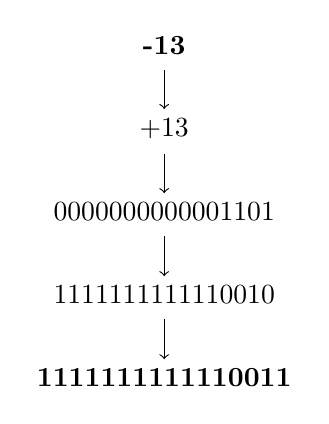
\begin{tikzpicture}[
node distance = 3em,
]
\node (n1) {\textbf{-13}};
\node [below of = n1] (n2) {+13};
\node [below of = n2] (n3) {0000000000001101};
\node [below of = n3] (n4) {1111111111110010};
\node [below of = n4] (n5) {\textbf{1111111111110011}};
\path[->,draw=black, shorten < = 2pt] (n1) -- (n2) ;
\path[->,draw=black, shorten < = 2pt] (n2) -- (n3) ;
\path[->,draw=black, shorten < = 2pt] (n3) -- (n4) ;
\path[->,draw=black, shorten < = 2pt] (n4) -- (n5) ;

\end{tikzpicture}
\end{figure}
\end{columns}
\end{frame}